
\section{Vergleich und Validierung der Modellleistung}


Im Folgenden wird der umfassende Lernprozess des DDPG-Modells dargestellt, wobei ein besonderes Augenmerk auf die ersten 10.000 Iterationen gelegt wird, wie in Abbildung \ref{fig:ddpg-learning-phases} zu sehen ist. Dieser Abschnitt des Trainings ist besonders aussagekräftig, da abgesehen von den divergierenden Modellen, alle anderen Modelle nahe am Optimum zu konvergieren scheinen.


\paragraph{Phase 1: Verifikation und Robustheit des DDPG-Modells}
Die erste Phase unserer Untersuchung dient der Verifikation der Leistungsfähigkeit und Robustheit des Deep Deterministic Policy Gradient (DDPG)-Modells im Kontext der Optimierung von DC-DC-Wandlern. Hierbei konzentrieren wir uns auf zwei Varianten des DDPG-Modells: ein einfacheres, schnell zu trainierendes Modell und ein fortgeschrittenes Modell mit komplexerer Architektur und längeren Trainingszeiten. Unser Hauptziel ist es, zu demonstrieren, dass das DDPG-Modell in der Lage ist, nahezu optimale Lösungen zu erzielen.

Um die Gültigkeit und Zuverlässigkeit unserer Modelle zu bestätigen, vergleichen wir die Ergebnisse des DDPG-Modells mit denen eines anderen bekannten Optimierungsverfahrens, das für seine hohe Leistung bekannt ist. Diese methodische Triangulation – die Approximation der Lösungen durch zwei grundlegend verschiedene Ansätze – soll nicht nur die Ähnlichkeit der Ergebnisse aufzeigen, sondern auch die Stärke und Anpassungsfähigkeit des DDPG-Modells in diesem speziellen Anwendungsbereich unterstreichen. Wir analysieren, wie sich eine einfache quadratische Belohnungsfunktion, die die Abweichung von der Zielspannung bestraft, auf die Performance dieser Modelle auswirkt und wie dies im Vergleich zu dem alternativen Optimierungsverfahren steht.

\paragraph{Phase 2: Anpassung der Bestrafungsfunktion und Erweiterung des Suchraums}
In der zweiten Phase unserer Untersuchung wurde die Belohnungsfunktion modifiziert, um eine ausgewogenere Reaktion auf Spannungsabweichungen zu erzielen. Wir haben zwei Ansätze kombiniert: Für Spannungsabweichungen über einem Schwellenwert von 1 wird eine quadratische Bestrafung angewendet, um auf größere Spannungsschwankungen stärker zu reagieren und so die Stabilität des Systems zu verbessern. Für Abweichungen unter diesem Schwellenwert wird eine Bestrafung basierend auf dem absoluten Wert vorgenommen, was das System sensibler für kleinere Spannungsabweichungen macht.

Zusätzlich wurde der Suchraum für die Optimierung erheblich erweitert, um eine breitere Palette von Konfigurationsmöglichkeiten zu erforschen. Der neue Suchraum erstreckt sich nun über deutlich größere Bereiche:
- Kp: 0 bis 1000
- Ki: 0 bis 100
- Kd: 0 bis 10

Diese Erweiterung des Suchraums soll aufzeigen, wie sich die Modelle, insbesondere die Bayesianische Optimierung, die bei großen Suchräumen bekannterweise Herausforderungen hat, im Vergleich zum DDPG-Modell verhalten. Es wird interessant zu beobachten sein, wie diese Änderungen die Leistung und Effektivität der Modelle beeinflussen, insbesondere in Bezug auf ihre Fähigkeit, mit größeren und komplexeren Konfigurationsräumen umzugehen.

\paragraph{Phase 3: Miniaturisierung}

In der dritten Phase unserer Untersuchung widmen wir uns der Miniaturisierung der Netzwerkmodelle. Unser Ziel ist es, die Fähigkeiten eines reduzierten Modells zu evaluieren und zu verstehen, wie es trotz geringerer Komplexität effektiv funktionieren kann. Diese Untersuchungen sind entscheidend, um das Potenzial der kompakten Modelle für den Einsatz in realen Anwendungsszenarien zu erkennen.

% \textbf{Erwartete Auswirkungen:}
% Durch diese Anpassung erwarten wir, dass die Modelle eine feinere Abstimmung der Spannungsregelung erlernen und gleichzeitig eine robustere Reaktion auf größere Spannungsschwankungen zeigen. Dieser Ansatz soll die Balance zwischen Sensitivität für geringfügige Abweichungen und effektiver Kontrolle über größere Störungen verbessern.


\section{Phase 1: Einfache und Fortgeschrittene Netzwerkmodelle}
\label{subsec:Basic_Advanced_Models}

In diesem Abschnitt werden die Ergebnisse der drei verschiedenen Ansätze zur Optimierung des DC-DC-Wandlers vorgestellt: die Bayesianische Optimierung sowie die kleinen und großen DDPG-Netzwerkmodelle. Die Belohnungen, die mit jeder Konfiguration erzielt wurden, bieten einen Einblick in die Effektivität jedes Ansatzes.

\paragraph{Hyperparameter}

\begin{table}[htbp]
\centering
\caption{Erweiterter Vergleich der Hyperparameter für das kleine und große DDPG-Modell unter Einbeziehung des Parameterraums}
\label{tab:extended_hyperparameters}
\begin{tabular}{lcc}
\hline
\textbf{Parameter} & \textbf{Kleines Modell} & \textbf{Großes Modell} \\
\hline
ALPHA & 0.001 & 0.0001 \\
WORKER & 12 & 12 \\
ITERATION & 1 & 1 \\
STEPS & 2000 & 20000 \\
BATCH\_SIZE & 72 & 250 \\
EXPLOITATION & 10 & 10 \\
LAYERS & 2 & 12 \\
LAYER\_1 & 158 & 158 \\
LAYER\_2 & 52 & 52 \\
NOISE & 0.3 & 0.45 \\
GAMMA & 0.0 & 0.0 \\
\textbf{Kp-Bereich} & 0 bis 10 & 0 bis 10 \\
\textbf{Ki-Bereich} & 0.0 bis 1.0 & 0.0 bis 1.0 \\
\textbf{Kd-Bereich} & 0.0 bis 0.2 & 0.0 bis 0.2 \\
\hline
\end{tabular}
\end{table}

\begin{figure}[htbp]
\centering
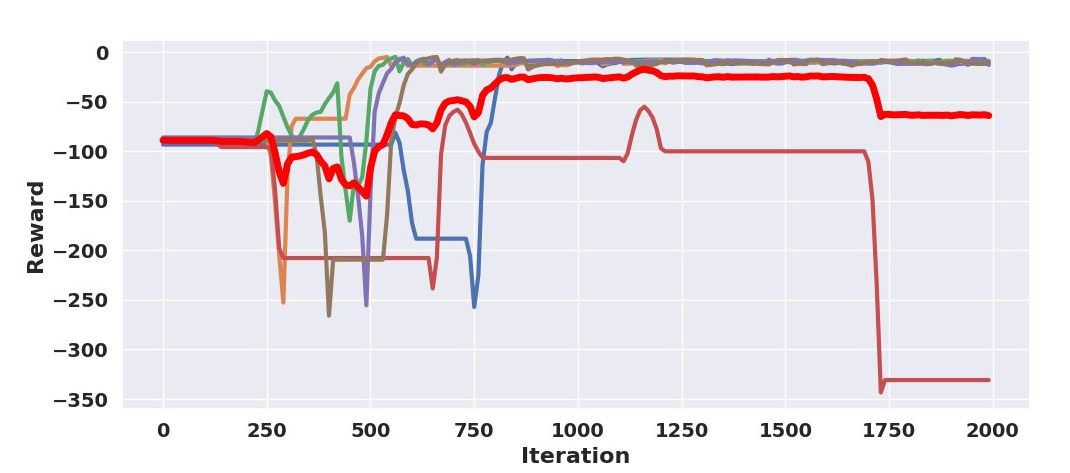
\includegraphics[width=0.7\textwidth]{4Ergebnisse/Phasen/1Phase/1Q_klein_epoch.png}
\caption{Belohnungsentwicklung über die Zeit für das kleine DDPG-Modell.}
\end{figure}

\begin{figure}[htbp]
\centering
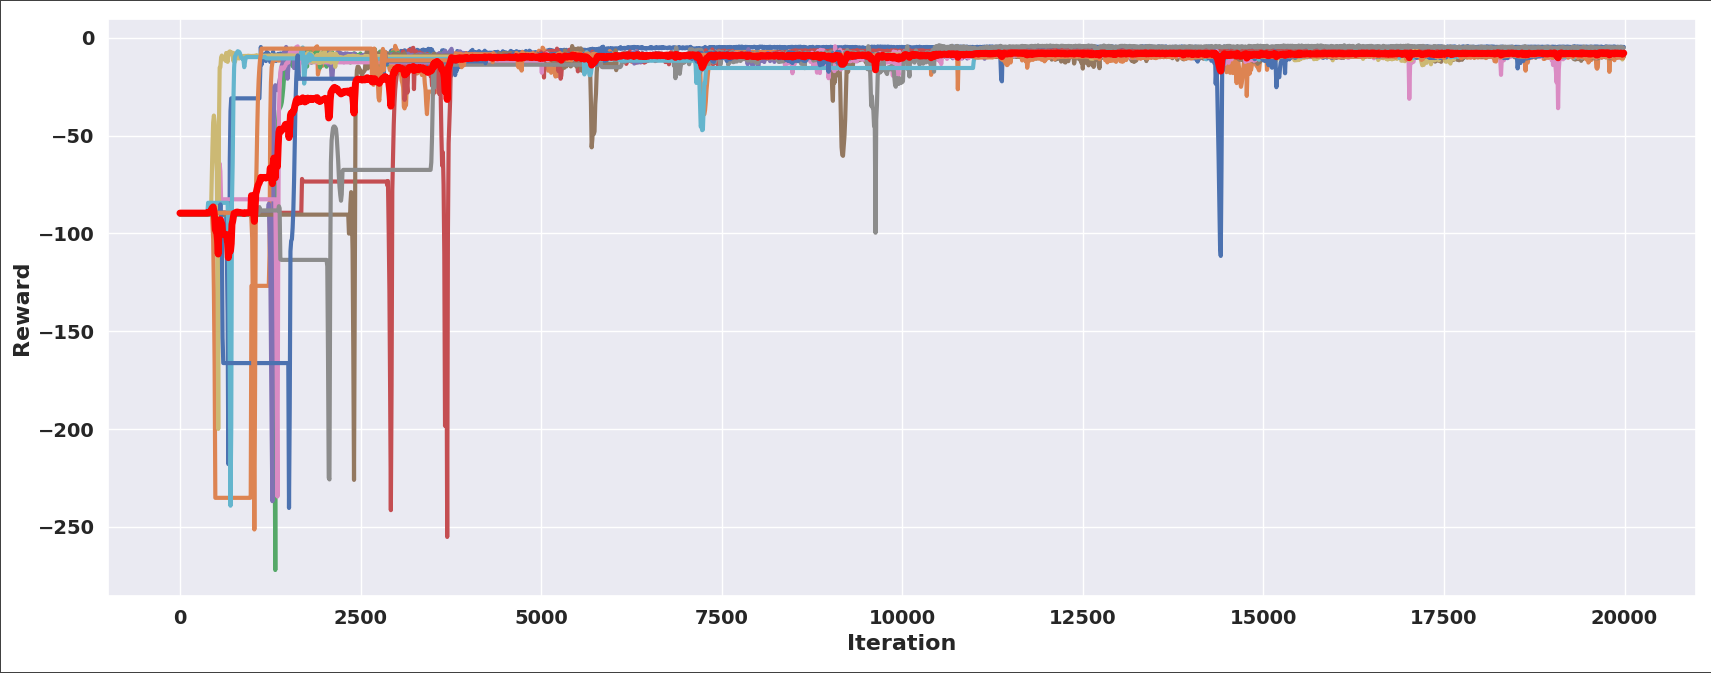
\includegraphics[width=0.92\textwidth,  trim=10px 10px 10px 10px, clip]{4Ergebnisse/Phasen/1Phase//1R_gross_epoch.png}
\caption{Belohnungsentwicklung über die Zeit für das große DDPG-Modell.}
\end{figure}


\begin{table}[htbp]
\centering
\caption{Vergleich der Ergebnisse verschiedener Modelle}
\label{tab:model_comparison}
\begin{tabular}{|c|c|c|}
\hline
\textbf{Modell} & \textbf{Ergebnis} & \textbf{Parameter} \\
\hline
Bayesian Optimization & -3.63 & 
\begin{tabular}[c]{@{}c@{}}Induktivität: 5.0e-3\\ Kapazität: 10.0e-6\\ Kp: 3.9250\\ Ki: 0.8521\\ Kd: 0.0139\end{tabular} \\
\hline
Kleines DDPG-Modell & -3.9098 & 
\begin{tabular}[c]{@{}c@{}}Induktivität: 5.0e-3\\ Kapazität: 10.0e-6\\ Kp: 2.4306\\ Ki: 0.6766\\ Kd: 0.0094\end{tabular} \\
\hline
Großes DDPG-Modell & -3.4217 & 
\begin{tabular}[c]{@{}c@{}}Induktivität: 5.0e-3\\ Kapazität: 10.0e-6\\ Kp: 3.4217\\ Ki: 0.6777\\ Kd: 0.0127\end{tabular} \\
\hline
\end{tabular}
\end{table}


\begin{figure}[htbp]
\centering
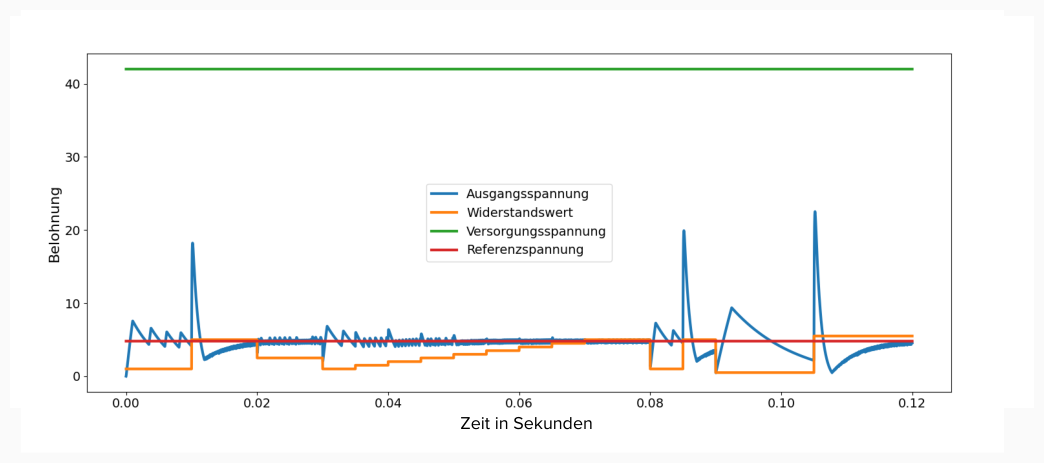
\includegraphics[width=0.99\textwidth, trim=10px 10px 10px 10px, clip]{4Ergebnisse/Phasen/1Phase/1S_small_search_space_bayes.png}
\caption{Darstellung des Regelungsverhaltens eines durch Bayes'sche Optimierung eingestellten PID-gesteuerten DC-DC-Konverters. Die Grafik zeigt die Belohnungsentwicklung über die Zeit und reflektiert die Anpassung der Ausgangsspannung (blau) an die Referenzspannung (rot) unter Berücksichtigung der Versorgungsspannung (grün) und des Widerstandswertes (orange). Die Ergebnisse verdeutlichen die Effektivität der Bayes'schen Optimierung bei der Feinabstimmung des Reglers für eine stabile Spannungsregelung.}
\label{fig:bayesian_optimization_pid_control}
\end{figure}
%
\begin{figure}[htbp]
\centering
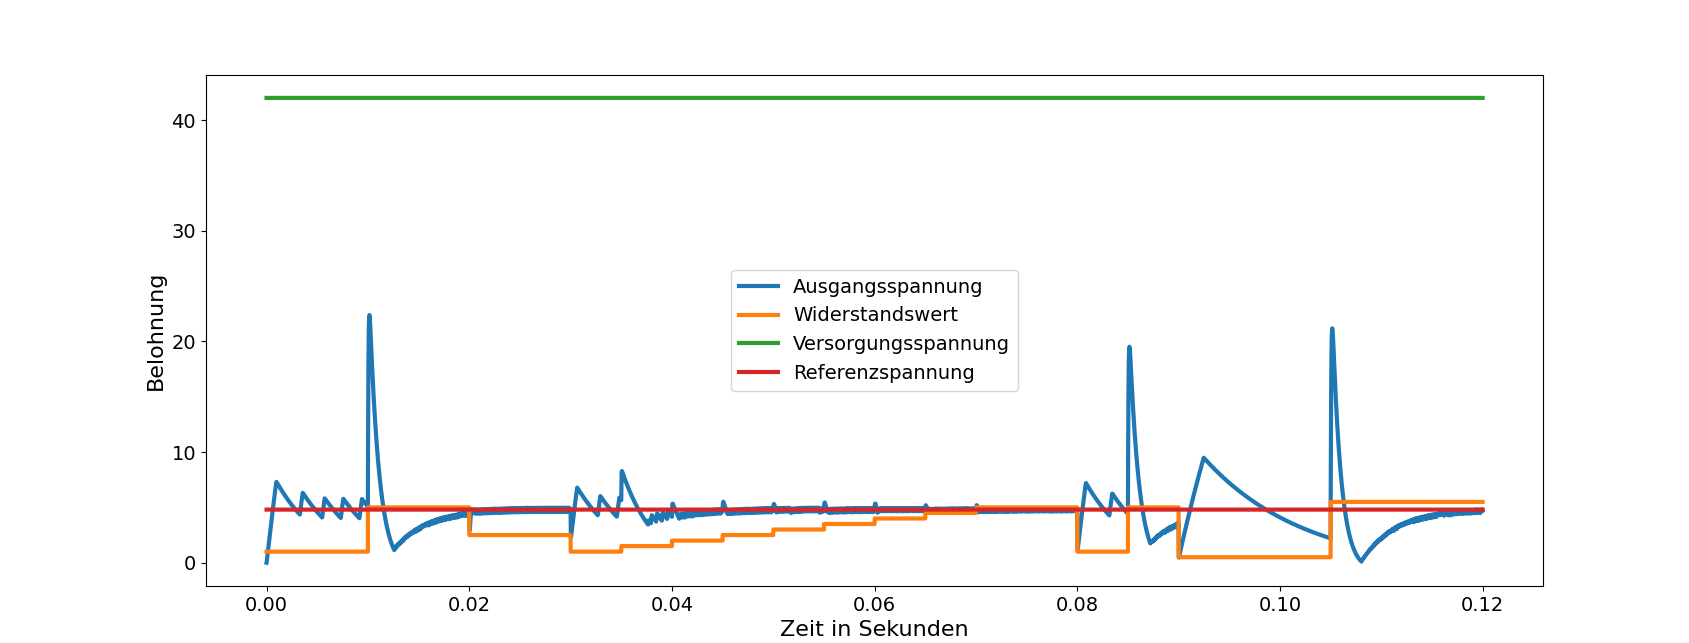
\includegraphics[width=0.99\textwidth]{4Ergebnisse/Phasen/1Phase//1T_small_search_space_small_net_dcdc.png}
\caption{Regelungsverhaltens über die Zeit für das kleine DDPG-Modell.}
\label{fig:small_ddpg_results}
\end{figure}
%
\begin{figure}[htbp]
\centering
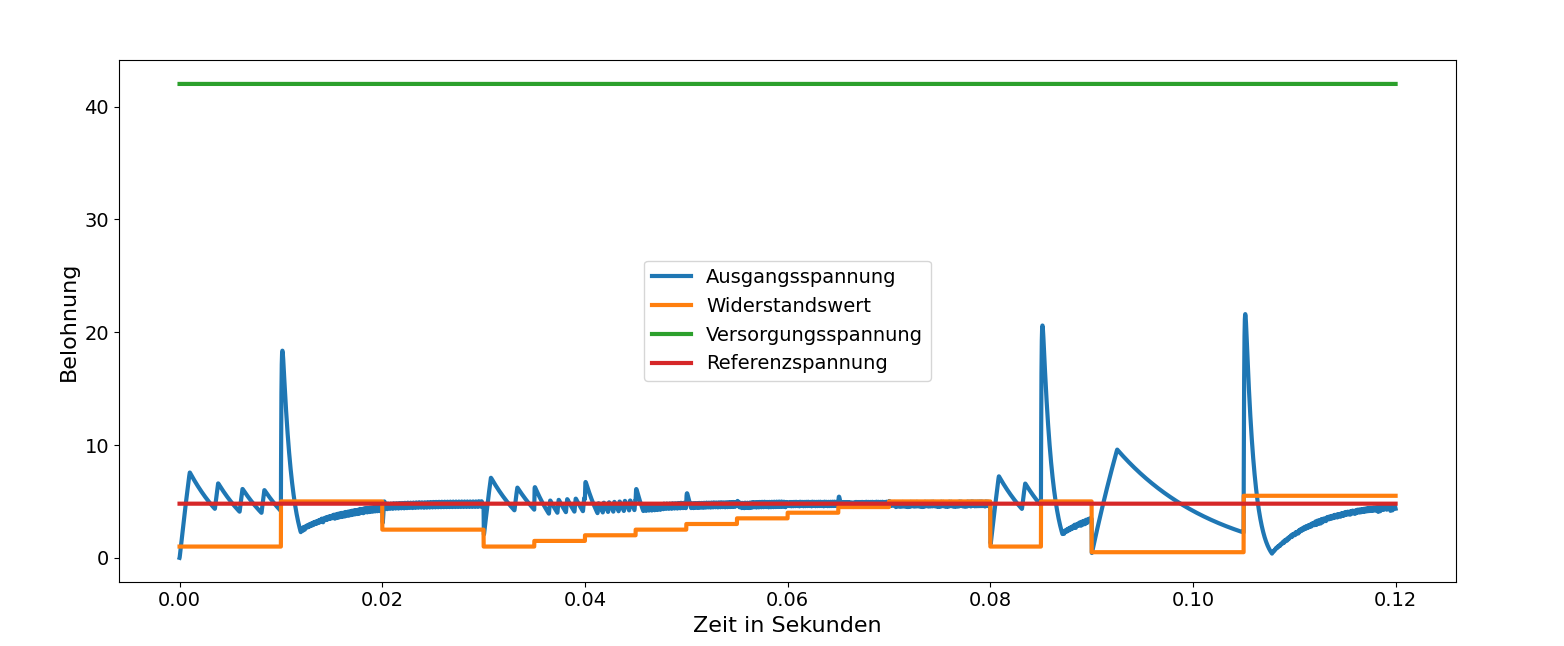
\includegraphics[width=0.99\textwidth]{4Ergebnisse/Phasen/1Phase//1U_big_net_dcdc.png}
\caption{Regelungsverhaltens über die Zeit für das große DDPG-Modell.}
\label{fig:large_ddpg_results}
\end{figure}

Die Abbildungen \ref{fig:bayesian_optimization_results}, \ref{fig:small_ddpg_results} und \ref{fig:large_ddpg_results} zeigen die jeweiligen Belohnungen, die durch die unterschiedlichen Optimierungsverfahren erzielt wurden.

\paragraph{Analyse der Ergebnisse: Leistungsvergleich der Optimierungsansätze}
Bei der Betrachtung der erzielten Ergebnisse aus den verschiedenen Optimierungsansätzen wird deutlich, dass sich die Leistungsdifferenzen vor allem im Belohnungswert (Reward) widerspiegeln. Alle drei Ansätze - Bayesianische Optimierung, kleines und großes DDPG-Modell - waren in der Lage, eine optimale oder nahezu optimale Lösung für die gestellte Aufgabe zu finden, wobei die Unterschiede in den tatsächlichen Spannungsverläufen minimal waren.

Interessanterweise zeigte das kleinere DDPG-Modell die geringste Leistung, was sich sowohl in niedrigeren Belohnungswerten als auch in einer weniger stabilen Konvergenz äußerte. Im Gegensatz dazu erreichte das große DDPG-Modell die besten Belohnungswerte, wobei alle Modelle eine gewisse Leichtigkeit bei der Konvergenz zeigten. Die Bayesianische Optimierung lag in ihrer Leistung dazwischen.

\paragraph{Synthese der Ergebnisse}

Interessanterweise zeigen sowohl die Bayesianische Optimierung als auch die DDPG-Modelle in ihren jeweiligen Anwendungen bemerkenswerte Übereinstimmungen in ihren Ergebnissen. Diese Konsistenz unterstreicht die Robustheit unserer Methoden und die Verlässlichkeit der erzielten Optimierungen. Trotz der unterschiedlichen Herangehensweisen und Techniken, die bei diesen beiden Methoden zum Einsatz kommen, konvergieren ihre Ergebnisse hin zu ähnlichen Lösungen. Dies deutet darauf hin, dass beide Ansätze effektiv die kritischen Bereiche des Parameterraums identifizieren und optimieren, was ein zentrales Ziel unserer Forschung ist.


\section{Phase 2: Vertiefte Analyse und Optimierung in Erweiterten Parameterräumen}
\label{subsec:Detailed_Learning_Process_Phase2}



\begin{table}[htbp]
\centering
\caption{Überblick über die Hyperparameter des DDPG-Modells inklusive Parameterraum}
\label{tab:hyperparameters_Phase2}
\begin{tabular}{lc}
\hline
\textbf{Parameter} & \textbf{Wert} \\
\hline
ALPHA & \( 1 \times 10^{-6} \) \\
WORKER & 6 \\
ITERATION & 1 \\
STEPS & 60000 \\
BATCH\_SIZE & 500 \\
EXPLOITATION & 10 \\
LAYERS & 24 \\
LAYER\_1 & 158 \\
LAYER\_2 & 52 \\
NOISE & 0.45 \\
GAMMA & 0.0 \\
MAX\_KP & 1000.0 \\
MAX\_KI & 100.0 \\
MAX\_KD & 10.0 \\
\hline
\end{tabular}
\end{table}

In dieser Phase unserer Untersuchung konzentrieren wir uns auf die vertiefte Analyse des Lernprozesses unter Berücksichtigung der modifizierten Belohnungsfunktion und der Erweiterung des Suchraums. Diese Phase ermöglicht es uns, ein detailliertes Verständnis dafür zu entwickeln, wie unsere Modelle auf diese Änderungen reagieren und sich anpassen.

\paragraph{Anpassung der Belohnungsfunktion}
Um eine differenziertere Reaktion auf Spannungsabweichungen zu erzielen, haben wir die Belohnungsfunktion angepasst. Für größere Abweichungen, spezifisch über einem Schwellenwert von 1, wird eine quadratische Bestrafung angewendet, um auf diese stärker zu reagieren. Dies verbessert die Stabilität des Systems bei größeren Spannungsschwankungen. Für kleinere Abweichungen, die unter diesem Schwellenwert liegen, wird eine Bestrafung auf Basis des absoluten Wertes vorgenommen. Dies macht das System sensibler für kleinere Spannungsabweichungen und ermöglicht eine feinere Justierung.

\paragraph{Erweiterung des Suchraums}
Wir haben den Suchraum erheblich erweitert, um eine größere Bandbreite an Konfigurationsmöglichkeiten zu erforschen. Dies erlaubt es uns, die Robustheit unserer Modelle in einem größeren und komplexeren Parameterraum zu testen. Insbesondere wollten wir untersuchen, wie die Bayesianische Optimierung, die in größeren Räumen typischerweise Herausforderungen begegnet, im Vergleich zum DDPG-Modell abschneidet. Diese Erweiterung hilft auch dabei, die Flexibilität und Anpassungsfähigkeit unserer Modelle in Szenarien mit weniger definierten Parametern zu demonstrieren.

\begin{figure}[htbp]
\centering
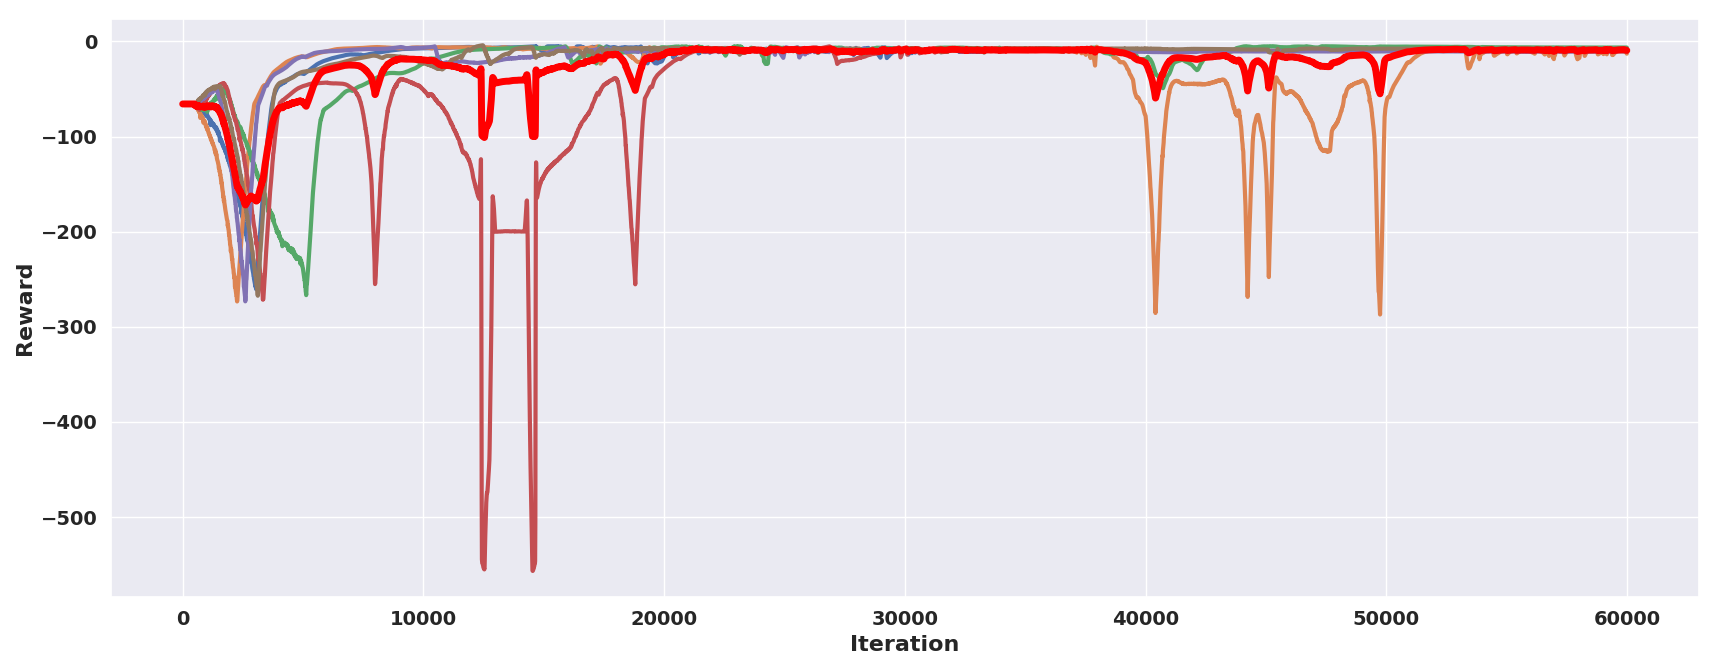
\includegraphics[width=\textwidth]{4Ergebnisse/Phasen/2Phase/2Phase.png}
\caption{Gesamtansicht des Lernprozesses des DDPG-Modells.}
\label{fig:phase 2 whole lern process}
\end{figure}

\paragraph{Detaillierte Darstellung des Lernprozesses}
Um die Entwicklung und Konvergenz unserer Modelle zu veranschaulichen, werden wir den Lernprozess detailliert darstellen, einschließlich visueller Darstellungen und Screenshots. Diese Darstellung soll den Fortschritt der Modelle im Laufe des Trainings verdeutlichen und zeigen, wie sie sich den neuen Herausforderungen stellen und anpassen. Durch die Kombination von modifizierter Belohnungsfunktion und erweitertem Suchraum können wir die Vielseitigkeit und Leistungsfähigkeit unserer Ansätze in einer breiten Palette von Anwendungsfällen aufzeigen. Während dieses Trainingsprozesses wurde eine beträchtliche Anzahl von Epochen genutzt. Die gewählte Lernrate war dabei bewusst gering gehalten, um eine stabile Konvergenz zu gewährleisten. Wie aus dem Graphen ersichtlich, haben die meisten Modelle eine signifikante und positive Konvergenz gezeigt, was auf die Effektivität des Lernansatzes und die ausgewählten Hyperparameter schließen lässt.




\begin{figure}[htbp]
\centering
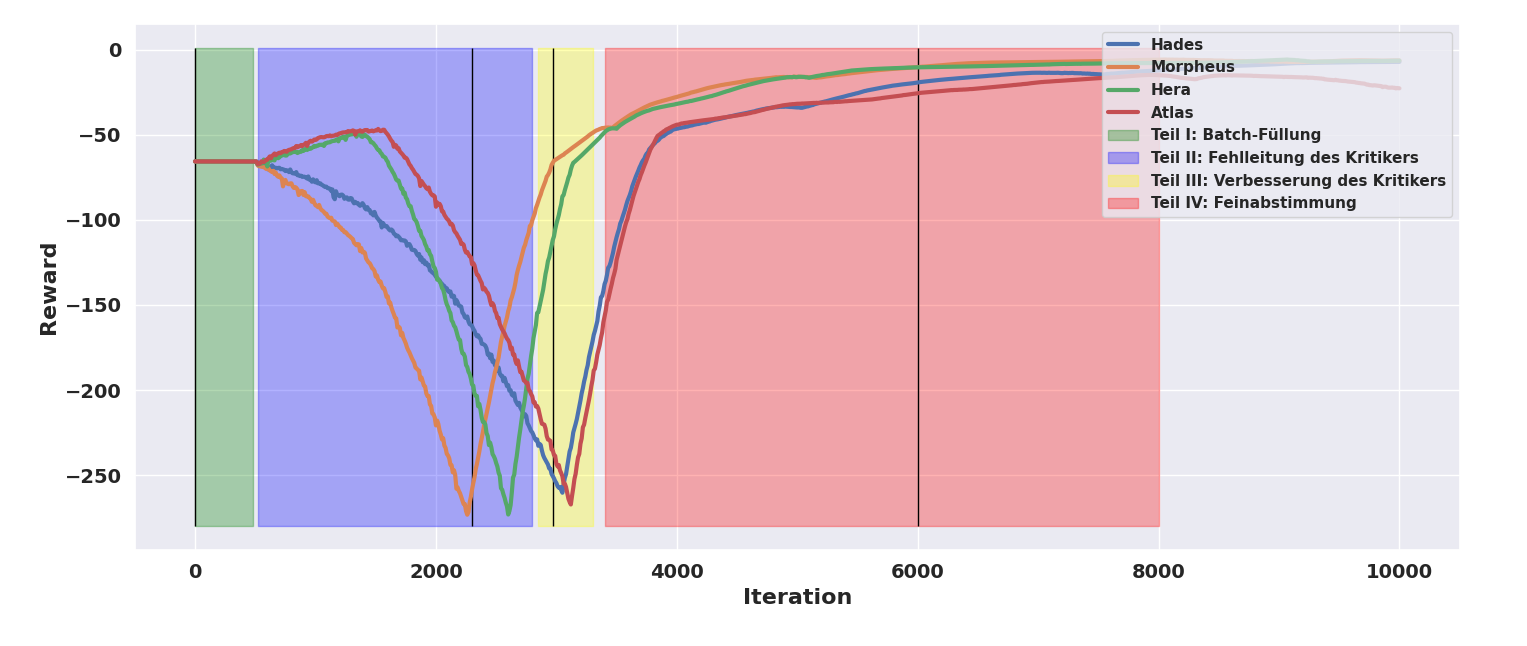
\includegraphics[width=\textwidth]{4Ergebnisse/Phasen/2Phase/4_0Presentation_of_Phase.png.png}
\caption{Detaillierte Darstellung der Lernprozesse und ausgewählten Stichproben in den verschiedenen Phasen des DDPG-Modells.}
\label{fig:ddpg-learning-phases}
\end{figure}

 Die initiale Selektion für die detaillierte Analyse fokussiert auf die Modelle, die zu Beginn des Trainings die besten Resultate aufweisen. Diese Vorauswahl basiert auf der Performance und der Konvergenzgeschwindigkeit in den ersten 10.000 Iterationen, wie Abbildung \ref{fig:ddpg-learning-phases} illustriert. Diese Modelle zeigen eine effektive Anpassung an den erweiterten Parameterraum und lassen auf ein optimiertes Lernverhalten schließen.


\subsection{Teil I. Anfängliche Lernprozesse und Batch-Füllung}
In Abbildung \ref{fig:ddpg-learning-phases} ist die erste Phase des Lernprozesses, markiert mit grün, deutlich zu erkennen. In dieser Phase zeigt sich ein flacher Verlauf der Lernkurven, was darauf zurückzuführen ist, dass der Batch zunächst gefüllt werden muss, bevor das eigentliche Lernen beginnen kann. Diese Anfangsphase ist essenziell, da wir hier den Stochastischen Gradientenabstieg (siehe Abschnitt:\ref{sec: Stochastisch Gredient Descent})  verwenden. Das Modell nutzt eine Vielzahl von Zustandsübergängen, um den Gradienten zu berechnen, was bedeutet, dass eine ausreichende Menge an Daten gesammelt werden muss, bevor eine Optimierung der Parameter effektiv stattfinden kann.


\begin{table}[htbp]
\centering
\caption{Stichprobe des Modells Morpheus bei Iteration 0}
\label{tab:sample_morpheus}
\begin{tabular}{l c}
\hline
\textbf{Parameter} & \textbf{Wert} \\
\hline
Iteration & 0 \\
Reward & -65.68 \\
Action & [500.00000022, 50.00000000, 4.99999991] \\
Induktivität & \( 5.0 \times 10^{-3} \) \\
Kapazität & \( 10.0 \times 10^{-6} \) \\
\hline
\end{tabular}
\end{table}

Ein weiterer interessanter Punkt, der in dieser Phase zu beobachten ist, betrifft die Ausgangswerte der Aktionen, die nahe bei [500, 50, 5] liegen. Dies ist auf die Aktivierungsfunktion zurückzuführen, die am Ende der 12 Schichten des Netzwerks angewendet wird. Da die Eingangswerte nicht normalisiert wurden und relativ klein sind, werden anfangs wahrscheinlich nur wenige Neuronen aktiviert, insbesondere unter Verwendung von Aktivierungsfunktionen wie ReLU, die das Überschreiten einer bestimmten Schwelle erfordern. Daraus folgt, dass die meisten Modelle anfänglich von ähnlichen Werten ausgehen, was eine Herausforderung für den Anfang des Lernprozesses darstellt.

\begin{figure}[htbp]
\centering
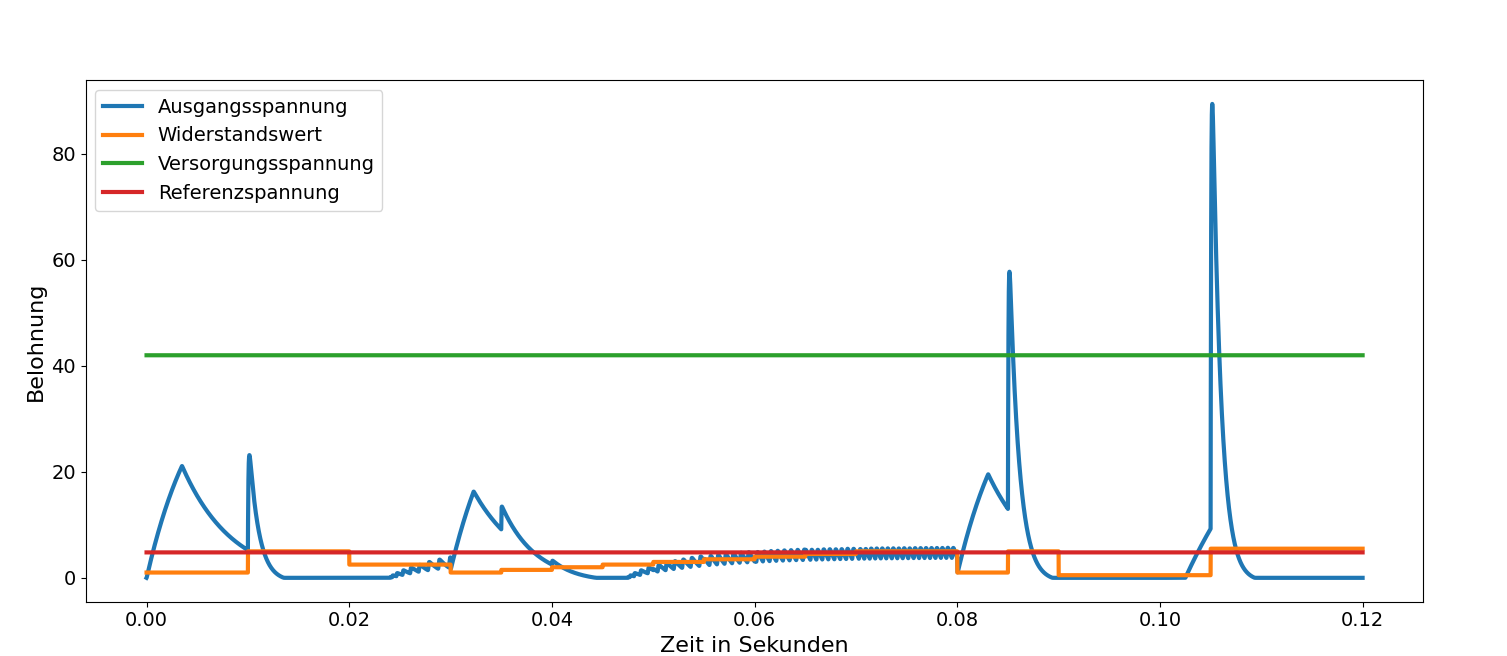
\includegraphics[width=\textwidth]{4Ergebnisse/Phasen/2Phase/5_I.png}
\caption{Stichprobe des Modells Morpheus bei Iteration 0 / Batchfüllung}
\label{fig:untrained}
\end{figure}


Die erste Stichprobe zeigt die Anfangsversuche des PID-Reglers, eine Regelung durchzuführen. Wie in Abbildung \ref{fig:untrained} erkennbar, gelingt es dem Regler noch nicht, die Ausgangsspannung effektiv zu stabilisieren. Die blaue Linie, die die Ausgangsspannung darstellt, haftet nicht an der roten Referenzlinie, was auf eine unzureichende Steuerung hinweist. Insbesondere bei großen Stromspitzen überschreitet die Spannung die Versorgungsspannung und erreicht Werte bis zu 90 Volt, manchmal fällt sie auch auf null ab. Dies würde normalerweise als suboptimales Regelverhalten eingestuft.

Trotzdem, wenn die Störungen nicht zu groß sind und dem System ausreichend Zeit gegeben wird, beginnt es, sich auf den gewünschten Wert einzupendeln, obwohl noch starke Oszillationen sichtbar sind. Dies deutet darauf hin, dass das System das Potenzial hat, sich zu stabilisieren, obwohl der aktuelle Regelungsansatz noch verbesserungsbedürftig ist.

\subsection{Teil II. Fehlleitung durch den Kritiker}
\label{subsec:Phase2_Misguidance_by_Critic}


\begin{table}[htbp]
\centering
\caption{Stichprobe des Modells Morpheus bei Iteration 2200}
\label{tab:sample_morpheus_2200}
\begin{tabular}{l c}
\hline
\textbf{Parameter} & \textbf{Wert} \\
\hline
Iteration & 2200 \\
Reward & -260.67 \\
Action & [514.42673523, 50.32317324, 4.64697339] \\
Induktivität & \( 5.0 \times 10^{-3} \) \\
Kapazität & \( 10.0 \times 10^{-6} \) \\
\hline
\end{tabular}
\end{table}


Die zweite Phase der Untersuchung offenbarte eine bemerkenswerte Dynamik zwischen dem Akteur und dem Kritiker. Während der Akteur begann, sein Verhalten basierend auf dem Feedback des Kritikers anzupassen, führten diese Änderungen zunächst zu keiner Verbesserung der Zielerreichung. Dies zeigte, dass der Akteur anfänglich den Empfehlungen eines noch nicht ausreichend trainierten Kritikers folgte, was zu suboptimalen Entscheidungen und einer Verschlechterung der Leistung gegenüber dem Referenzwert führte. Der signifikante Abfall des Rewards und die extremen Ausschläge der Ausgangsspannung, die in Abbildung \ref{fig:phase_ii_morpheus} dargestellt sind, verdeutlichen die Konsequenzen der Fehlleitung. Die Ausgangsspannung erreichte Spitzen von bis zu 250 Volt, was in der realen Anwendung wahrscheinlich zu einer Überlastung des Systems geführt hätte. Diese Phase illustriert, wie kritisch es ist, dass der Kritiker präzise und zuverlässige Rückmeldungen liefert, um eine effektive Anpassung des Akteurs zu gewährleisten.Diese Beobachtungen wurden durch die Stichprobe des Modells Morpheus bei Iteration 2200 untermauert, wie in Tabelle \ref{tab:sample_morpheus_2200} dargestellt.


\begin{figure}[htbp]
\centering
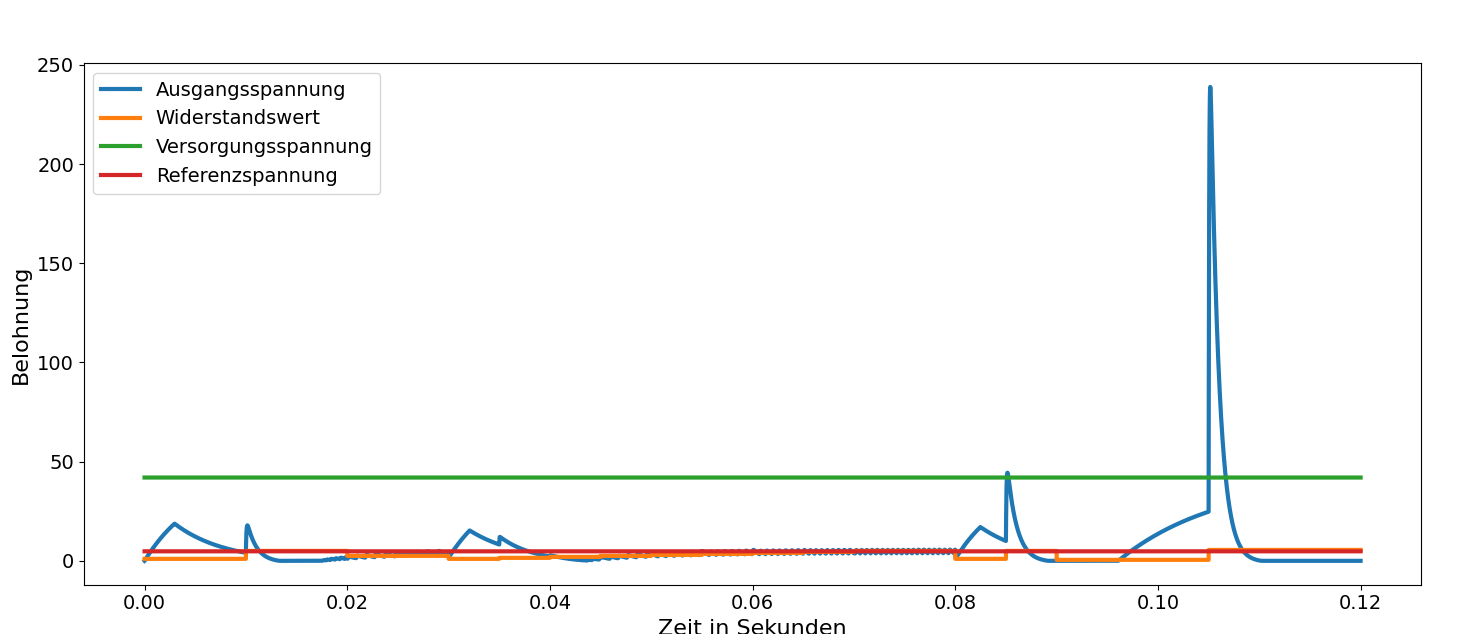
\includegraphics[width=\textwidth]{4Ergebnisse/Phasen/2Phase/TEilII_2.png}
\caption{Auffällige Abweichungen im Regelverhalten des Modells Morpheus während Phase II.}
\label{fig:phase_ii_morpheus}
\end{figure}


\subsection{Teil III. Feinjustierung und Konvergenz in Richtung Optimum}
\label{subsec:Fine_Tuning_and_Convergence_Towards_Optimum}

Mit fortschreitendem Training begann der Kritiker jedoch, die Lage korrekter einzuschätzen, und seine Bewertungen wurden zunehmend präziser. In der dritten Phase konnte beobachtet werden, wie der Akteur endlich begann, die angemessenen Anpassungen vorzunehmen, was zu einer allmählichen Verbesserung und Annäherung an die optimale Lösung führte. Die Richtung der Anpassungen stimmte nun mit den tatsächlichen Bewertungen des Kritikers überein, was zu einer iterativen Verbesserung des Gesamtverhaltens führte und den Lernprozess in die richtige Richtung lenkte.


Nachdem das Modell Morpheus 3000 Iterationen durchlaufen hatte, begann es, deutliche Fortschritte in der Regelungsleistung zu zeigen. Die vom Kritiker geleiteten Anpassungen des Akteurs führten zu einer bemerkenswerten Verbesserung der Belohnungswerte, was eine gezielte Annäherung an die gewünschte Referenzspannung mit einer verringerten Oszillationsamplitude signalisiert. Die Daten in Tabelle \ref{tab:sample_morpheus_3000} und die zugehörigen Regelungsausschläge in Abbildung \ref{fig:phase_iii_morpheus} legen nahe, dass trotz der gelegentlich über 100 Volt hinausgehenden Spitzenwerte die Regelungsstrategie des Akteurs die richtige Richtung einschlägt.

Die Bedeutung der Belohnungsfunktion in diesem Prozess kann nicht genug betont werden. Obwohl die PID-Koeffizienten andere Werte aufweisen als in der anfänglichen Lernphase, führt die Feinjustierung der Belohnungsfunktion zu einem Verhalten, das in seiner Leistung fast dem der ersten Phase entspricht. Es ist faszinierend zu sehen, wie das System trotz veränderter PID-Konfiguration zu einem ähnlichen Ausgangsverhalten konvergiert, was die Wichtigkeit und Wirksamkeit der Belohnungsfunktion in der Lernstrategie unterstreicht.

\begin{table}[htbp]
\centering
\caption{Stichprobe des Modells Morpheus bei Iteration 3000}
\label{tab:sample_morpheus_3000}
\begin{tabular}{l c}
\hline
\textbf{Parameter} & \textbf{Wert} \\
\hline
Iteration & 3000 \\
Belohnung & -64.33275232194337 \\
Aktion & [535.75499356, 51.67935919, 4.21606518] \\
Induktivität & \( 5.0 \times 10^{-3} \) \\
Kapazität & \( 10.0 \times 10^{-6} \) \\
\hline
\end{tabular}
\end{table}

\begin{figure}[htbp]
\centering
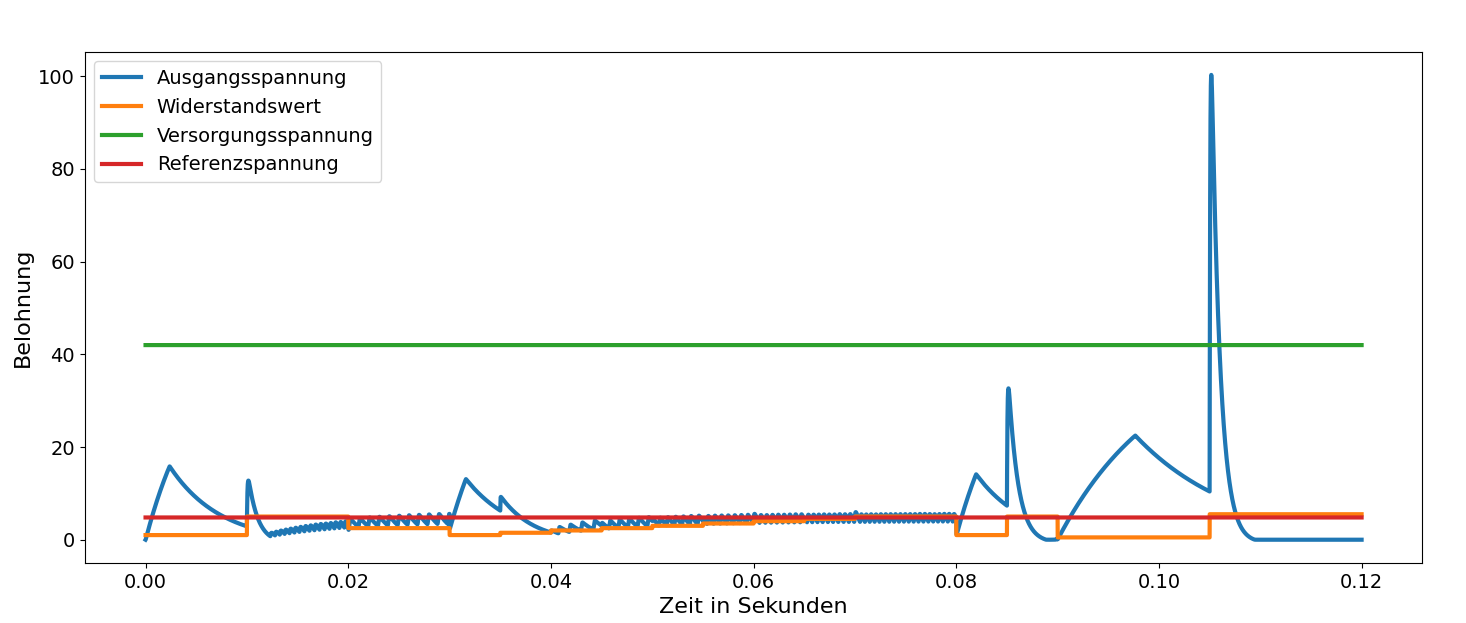
\includegraphics[width=\textwidth]{4Ergebnisse/Phasen/2Phase/TeilIII_2.png}
\caption{Verbesserung der Regelungsleistung des Modells Morpheus während der dritten Phase, illustriert durch die Annäherung der Ausgangsspannung an die Referenzspannung und die Verringerung der Oszillationen.}
\label{fig:phase_iii_morpheus}
\end{figure}


\subsection{Teil IV. Fortgeschrittene Konvergenz und Feinabstimmung}
\label{subsec:Advanced_Convergence_and_Fine_Tuning}


Die vierte und letzte Phase des Lernprozesses zeichnete sich durch eine langsame, aber stetige Annäherung des Akteurs an das Optimum aus \ref{fig:advanced_convergence_morpheus}. Die Verhaltensänderungen wurden feiner und gezielter, was darauf hindeutet, dass das Modell begann, die subtilen Nuancen der Umgebung zu verstehen und seine Aktionen entsprechend anzupassen. Es war ein langsamer Prozess der Verfeinerung, der darauf abzielte, die optimalen Einstellungen zu finden. Interessanterweise war in dieser Phase auch eine gelegentliche Divergenz bei einem der Agenten zu beobachten. \ref{fig:phase 2 whole lern process} Dies könnte darauf hinweisen, dass trotz der allgemeinen Tendenz zur Konvergenz immer noch das Potential für Instabilitäten oder für das Erkunden von neuen, unerwarteten Lösungspfaden bestand.


\begin{table}[htbp]
\centering
\caption{Stichprobe des Modells Morpheus bei Iteration 6000}
\label{tab:sample_morpheus_6000}
\begin{tabular}{l c}
\hline
\textbf{Parameter} & \textbf{Wert} \\
\hline
Iteration & 6000 \\
Belohnung & -10.21 \\
Aktion & [634.09879804, 55.28446324, 2.65851244] \\
Induktivität & \( 5.0 \times 10^{-3} \) \\
Kapazität & \( 10.0 \times 10^{-6} \) \\
\hline
\end{tabular}
\end{table}

Mit weiteren Fortschritten im Trainingsprozess erreicht das Modell Morpheus nach 6000 Iterationen eine Phase, in der eine signifikante Konvergenz erkennbar ist. Die Belohnungswerte verbessern sich weiter, und die Ausgangsspannung nähert sich stabil der Referenzspannung an, ohne die Versorgungsspannung zu überschreiten \ref{fig:advanced_convergence_morpheus}. Die Daten in Tabelle \ref{tab:sample_morpheus_6000} zeigen, dass die Anpassungen des Akteurs zu einer angemessenen Regelungsleistung führen und die Oszillationen der Spannungswerte minimiert werden. Die Ergebnisse dieser Phase sind vielversprechend und lassen auf eine erfolgreiche Anpassung des Modells schließen.

\begin{figure}[htbp]
\centering
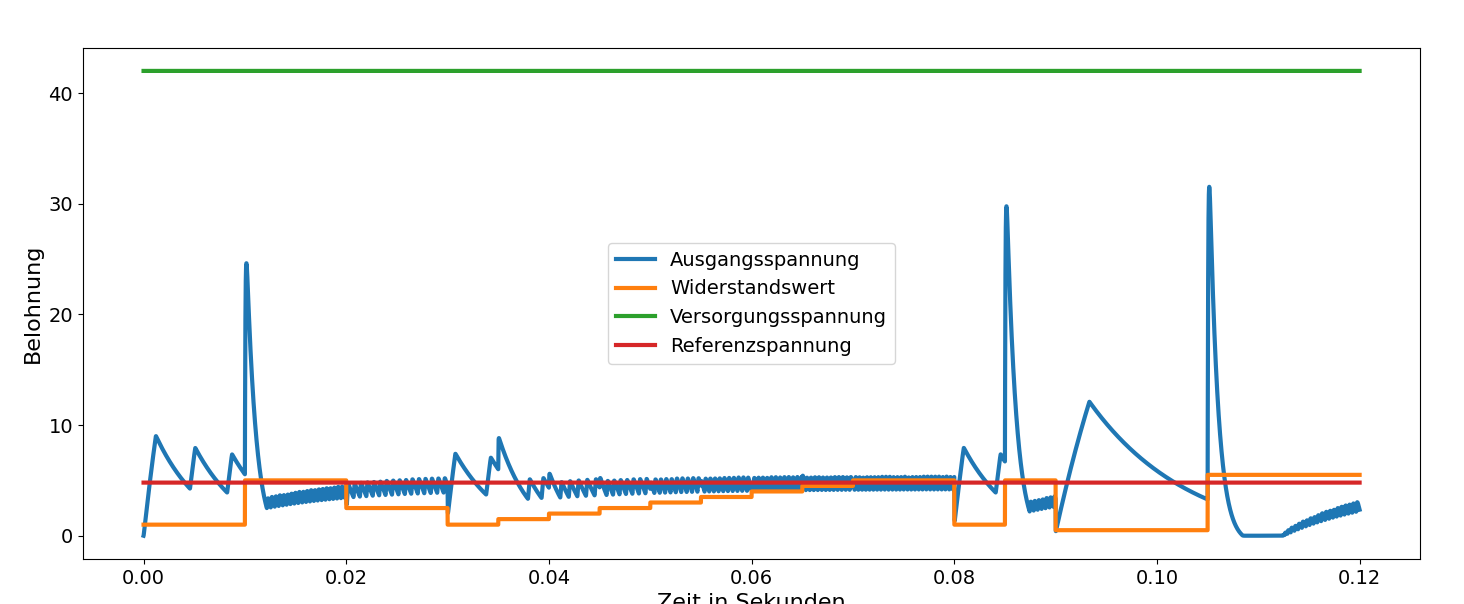
\includegraphics[width=\textwidth, trim=12px 12px 12px 12px, clip]{4Ergebnisse/Phasen/2Phase/TeilIV.png}
\caption{Die fortgeschrittene Konvergenz des Modells Morpheus mit einer sichtbaren Verbesserung der Regelungsleistung. }
\label{fig:advanced_convergence_morpheus}
\end{figure}

\subsection{Teil V. Erzielung einer nahezu optimalen Regelungsleistung}
\label{subsec:Achievement_of_Near-Optimal_Control_Performance}

Während der entscheidenden Endphase des Trainingsprozesses verzeichneten wir bei einem unserer Modelle, welches wir im Folgenden als Modell X bezeichnen, eine stetige Verbesserung der Regelungsleistung. Diese Beobachtung wird durch die in Abbildung \ref{fig:phase 2 whole lern process} dokumentierte, kontinuierliche Leistungssteigerung bestätigt. Durch konsequente Feinabstimmung und die Auswahl der leistungsfähigsten Modelle zu verschiedenen Zeitpunkten des Trainings konnte ein herausragendes Ergebnis erzielt werden: Das Modell X erreichte eine maximale Belohnung von -3.99. Dies deutet auf eine Performance hin, die dem optimalen Steuerungsverhalten sehr nahekommt.

\begin{table}[htbp]
\centering
\caption{Maximale Leistung des Modells X nach umfangreichen Trainingsiterationen}
\label{tab:maximum_performance_model_x}
\begin{tabular}{l c}
\hline
\textbf{Parameter} & \textbf{Wert} \\
\hline
Iteration & Geschätzt \\
Belohnung & -3.9928830028461824 \\
Aktion & [434.82286483, 91.83493555, 1.52657181] \\
Induktivität & \( 5.0 \times 10^{-3} \) \\
Kapazität & \( 10.0 \times 10^{-6} \) \\
\hline
\end{tabular}
\end{table}

\begin{figure}[htbp]
\centering
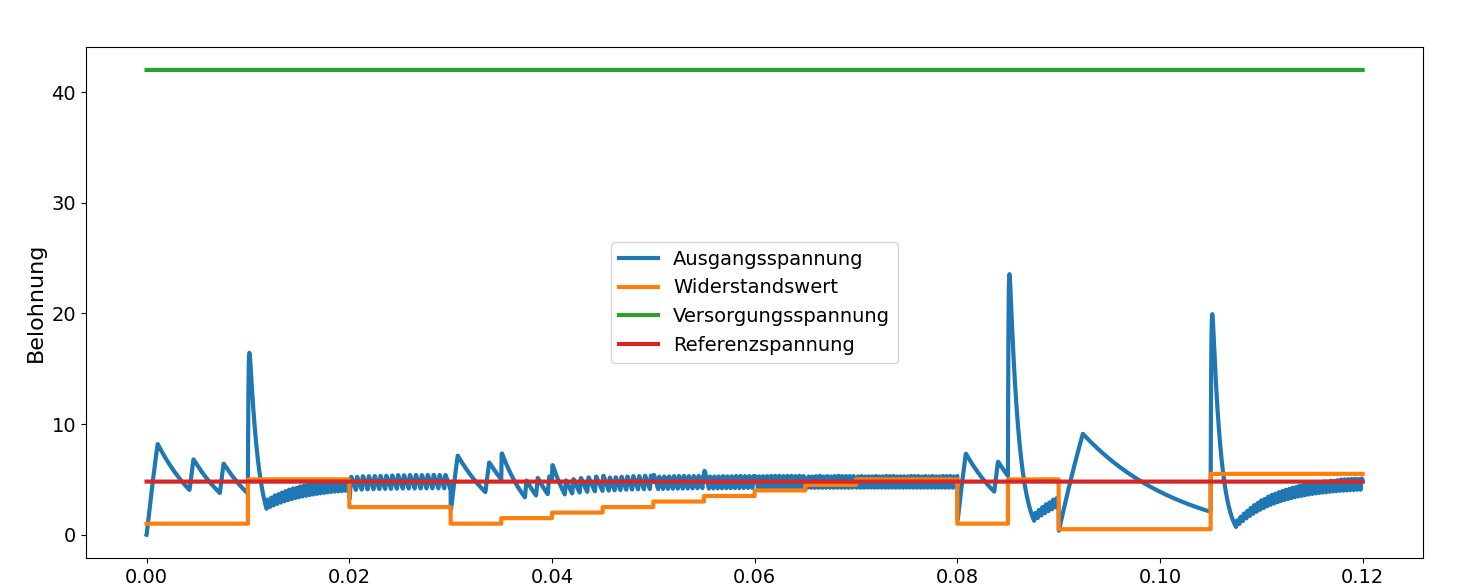
\includegraphics[width=\textwidth]{4Ergebnisse/Phasen/2Phase/TeilV.png}
\caption{Darstellung der finalen Leistungssteigerung des Modells X, welche die nahezu optimale Regelungsleistung illustriert.}
\label{fig:final_performance_model_x}
\end{figure}

Die Erreichung einer solch hohen Belohnung nach einer langen Reihe von Trainingsiterationen bestätigt die Effektivität unseres Ansatzes zur Modelloptimierung. Die Performance \ref{fig:final_performance_model_x} von Modell X stellt einen bedeutenden Meilenstein dar, der zeigt, dass das Modell nicht nur theoretisch, sondern auch in der simulierten Anwendung in der Lage ist, sich effektiv anzupassen und zu optimieren. Dieses Ergebnis betont die Relevanz und Präzision unserer Belohnungsfunktion sowie die Robustheit des DDPG-Modells unter komplexen und anspruchsvollen Bedingungen.


\subsection{Synthese der Ergebnisse}
\label{sec:Synthesis_of_Results}


\paragraph{Dynamik zwischen Akteur und Kritiker}
Die Interaktion zwischen Akteur und Kritiker, insbesondere in der zweiten Phase, zeigte die Komplexität des Lernprozesses auf, bei dem die Anfälligkeit für Fehlleitung ohne angemessene Leitung evident wurde.

\paragraph{Konvergenz und Feinjustierung}
Die dritte Phase demonstrierte, dass trotz anfänglicher Fehltritte der Algorithmus fähig ist, sich anzupassen und zu verbessern, was sich in einer konstanten Annäherung an die gewünschte Leistung manifestierte.

\paragraph{Erreichen einer hohen Leistung}
Die letzte Phase unterstrich die Potenz des Algorithmus, auch unter längeren und anspruchsvollen Trainingsbedingungen eine nahezu optimale Regelungsleistung zu erzielen, was durch das Modell X hervorragend dargestellt wurde.



\section{Phase 3: Miniaturisierung und Leistungsanalyse}
\label{subsec:Network_Miniaturization_Performance_Analysis}


\begin{table}[htbp]
\centering
\caption{Konfiguration und Ergebnisse des miniaturisierten Modells}
\label{tab:miniaturization_results}
\begin{tabular}{lc}
\hline
\textbf{Parameter} & \textbf{Wert} \\
\hline
ALPHA & \( 1 \times 10^{-5} \) \\
WORKER & 10 \\
ITERATION & 1 \\
STEPS & 30000 \\
BATCH\_SIZE & 250 \\
EXPLOITATION & 10 \\
LAYERS & 3 \\
LAYER\_1 & 10 \\
LAYER\_2 & 3 \\
NOISE & 0.4 \\
GAMMA & 0.0 \\
\hline
Maximale Belohnung & -4.29 \\
Entsprechende Aktion & [6.84119821, 0.75633377, 0.02226542] \\
\hline
\end{tabular}
\end{table}

Die Ergebnisse der Miniaturisierung sind bemerkenswert, da das verkleinerte Modell eine maximale Belohnung von -4.295256034278478 erreichte, was auf eine nahezu optimale Regelungsleistung hindeutet. Die entsprechenden Aktionen und detaillierten Konfigurationen des Modells sind in Tabelle \ref{tab:miniaturization_results} aufgeführt.

\begin{figure}[htbp]
\centering
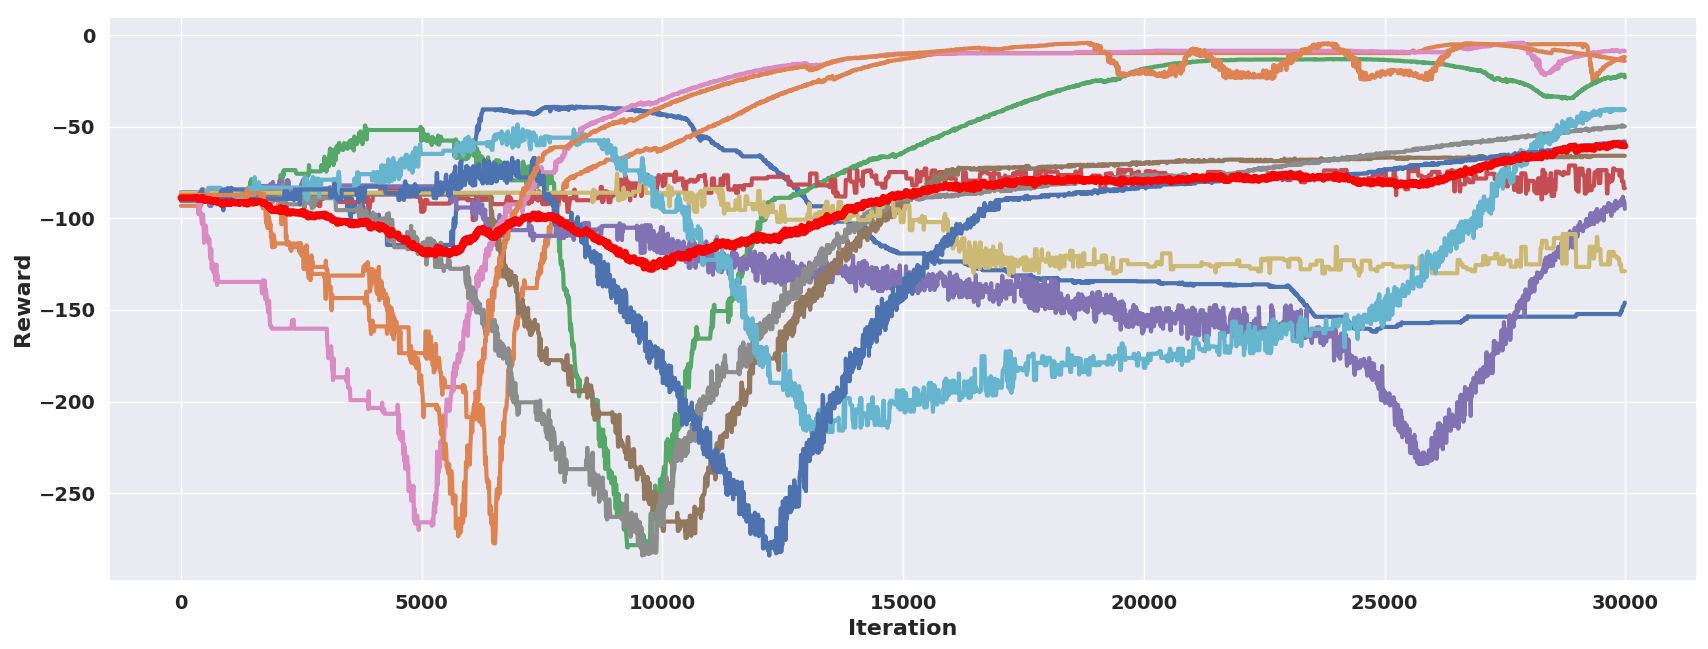
\includegraphics[width=\textwidth]{4Ergebnisse/Phasen/3Phase/3R_big_training_minimize_epoch.png}
\caption{Leistungskurve des miniaturisierten Modells über die Trainingsdauer.}
\label{fig:miniaturized_model_performance}
\end{figure}

Die Leistung des miniaturisierten Modells, wie in Abbildung \ref{fig:miniaturized_model_performance} gezeigt, demonstriert eindrucksvoll, dass eine effiziente Modellminiaturisierung ohne erheblichen Leistungsverlust möglich ist. Diese Erkenntnis ist besonders relevant für praxisnahe Anwendungen, wo kompakte Modelle aufgrund von 
Ressocenbe- schränkungen bevorzugt werden.

Die Ergebnisse wurden durch eine Kombination aus niedriger Lernrate und einer hohen Anzahl von Trainingsepochen erzielt. Die erzielten Ergebnisse \ref{fig:miniaturized_model_performance} weisen darauf hin, dass das Modell trotz der frühzeitigen Beendigung des Trainings bereits eine beachtliche Leistung demonstrierte. Dies legt nahe, dass mit einer Fortsetzung des Trainingsprozesses und einer weiteren Feinabstimmung der Hyperparameter möglicherweise noch höhere Performanzwerte hätten erreicht werden können. Die vorliegenden Ergebnisse bestätigen somit nicht nur die Effektivität des eingesetzten Trainingsansatzes, sondern auch das Potenzial für weitergehende Verbesserungen und Optimierungen.

Ein weiterer wichtiger Aspekt ist das Risiko des Overfittings bei komplexeren Modellen, wie bereits in Kapitel \ref{sec: overfitting} diskutiert. Overfitting tritt auf, wenn ein Modell zu sehr auf die spezifischen Trainingsdaten ausgerichtet ist und dadurch seine Fähigkeit verliert, auf neue, unbekannte Daten angemessen zu reagieren. Es ist eine bekannte Tatsache, dass einfachere Modelle häufig eine bessere Generalisierungsfähigkeit aufweisen, da sie weniger anfällig für das Auswendiglernen spezifischer Trainingsdaten sind. Unsere Ergebnisse zeigen, dass das miniaturisierte Modell trotz seiner Einfachheit eine gute Leistung erbringen konnte, was die Wichtigkeit einer ausgewogenen Modellkomplexität in der Modellentwicklung hervorhebt. 

Insgesamt legen diese Beobachtungen nahe, dass es vorteilhaft sein kann, sich auf die Optimierung von Hyperparametern zu konzentrieren, um kleinere, aber leistungsfähige Modelle zu entwickeln.


